\section{(6 points)}

Le tableau suivant, extrait d'une feuille d'un tableur, donne le prix annuel moyen du paquet de cigarettes (20 cigarettes) le plus vendu, en euros, entre 2000 et 2004.

\begin{center}
	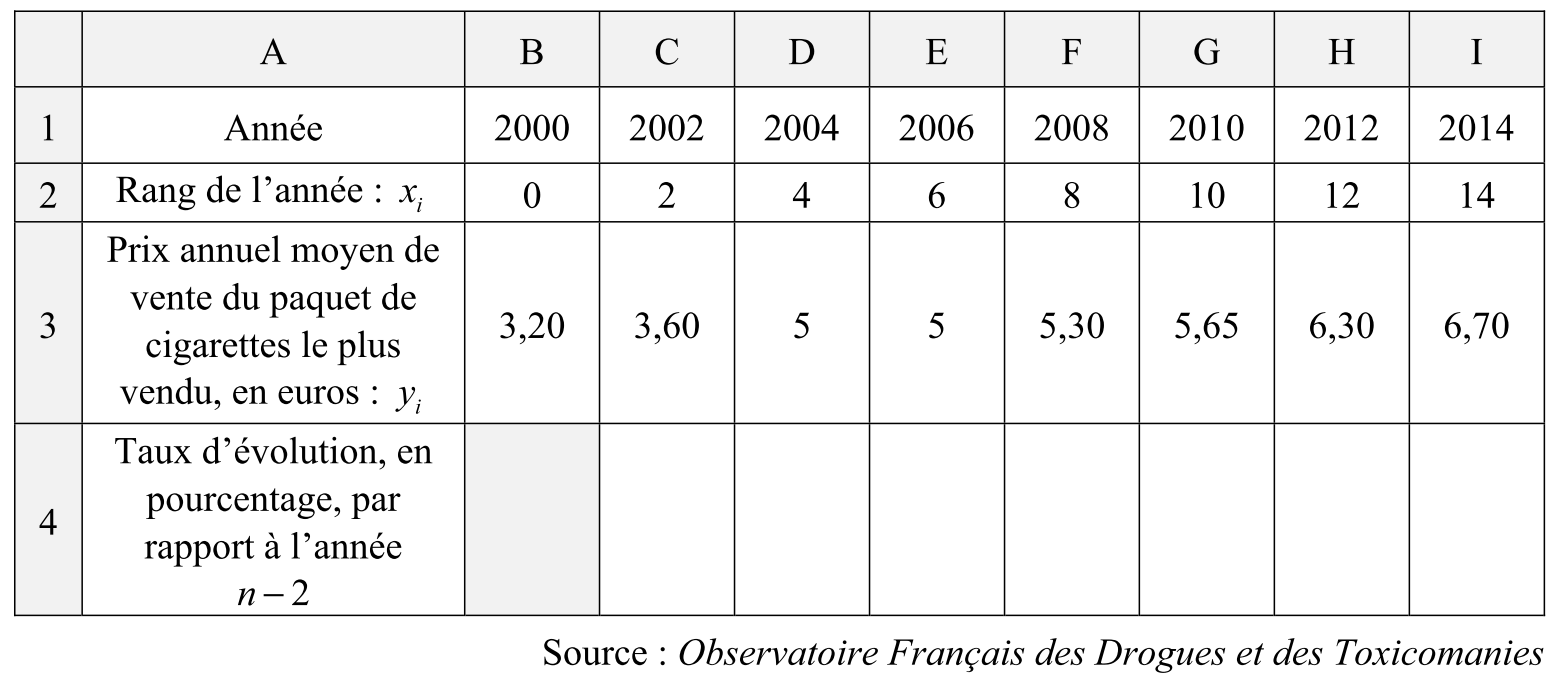
\includegraphics[scale=0.4]{img/tabac}
\end{center}

\subsection{(2 points)}

\begin{questions}
	\question[1] Un journaliste affirme que le prix entre 2000 et 2014 a augmenté de $50$ \%. L'affirmation est-elle vraie ou fausse ? Justifier.
	\begin{solution}
		Calcul de l'évolution du prix entre 2000 et 2014 :
		\begin{eqnarray*}
			t &=& \dfrac{v_{arrivée} - v_{départ}}{v_{départ}} \\
			t &=& \dfrac{6,70 - 3,20}{3,20} \\
			t &\approx& 1,09
		\end{eqnarray*}
	
	Entre 2000 et 2014 le prix moyen du paquet de tabac a augmenté d'environ 109 \%, donc l'affirmation est fausse.
	\end{solution}
	\question[1] La ligne 4 est au format pourcentage. Quelle formule peut-on saisir dans la cellule $C4$ et recopier vers la droite pour compléter la ligne 4 ?
	\begin{solution}
		Formule à saisir en en C4 :
		$=(C3-B3)/B3$
	\end{solution}
\end{questions}

\subsection{(4 points)}

\begin{questions}
	\question[2]
	
		\begin{parts}
			\part[1] Sur la feuille de papier millimétré fournie et à rendre avec la copie, représenter le nuage de points de coordonnées $(x_i;y_i)$ dans un repère orthogonal en choisissant :
			\begin{itemize}
				\item 1cm pour 2 années en abscisse ;
				\item 1cm pour 1 euro en ordonnée.
			\end{itemize}
		
			\part[1] Calculer les coordonnées du point moyen $G$ du nuage de points, puis placer le point $G$ sur le graphique précédent. Arrondir les résultats à \num{0.01} près.
			\begin{solution}
				Calcul des coordonnées du point moyen G :
				
				\begin{eqnarray*}
					\bar{x} &=& \dfrac{0 + 2 + 4 + 6 + 8 + 10 + 12 + 14}{8} \\
					\bar{x} &=& 7 \\ 
					& & \\
					%& & \\
					\bar{y} &=& \dfrac{3,20 + 3,60 + 5 + 5 + 5,30 + 5,65 + 6,30 + 6,70}{8} \\
					\bar{y} & \approx & 5,09
				\end{eqnarray*}
			
			Donc les coordonnées du point G sont $(7;5,09)$.
			\end{solution}
		\end{parts}
	
	\question[2] On admet que la droite $D$ d'équation $y=\num{0.24}x+\num{3.41}$ est un bon ajustement affine du nuage de points et que cet ajustement reste valable jusqu'en 2025.
		\begin{parts}
			\part[\half] Vérifier que le point $G$ appartient à la droite $D$.
			\begin{solution}
				\begin{eqnarray*}
					y &=& 0,24 x + 3,41 \\
					y &=& 0,24 \times 7 + 3,41 \\
					y &=& 5,09
				\end{eqnarray*}
			
			Donc le point $G$ appartient à la droite $D$.
			\end{solution}
		
			\part[\half] Tracer la droite $D$ sur le graphique précédent en indiquant les points utilisés.
			\begin{solution}
				
				\begin{eqnarray*}
					%y &=& 0,24 x + 3,41 \\
					y &=& 0,24 \times 0 + 3,41 \\
					y &=& 3,41
				\end{eqnarray*}
			
			Le point $A (0;3,41)$ appartient à la droite $D$. 
			
			ON peut tracer la droite $D$ à partir des points $A$ et $G$.
			\end{solution}
			\part[\half] Selon cet ajustement, quel sera le prix moyen annuel d'un paquet de cigarettes en France en 2020 ?
			\begin{solution}
				2020 est l'année de rang 20 (2020 - 2000 = 20) :
				
				\begin{eqnarray*}
					%y &=& 0,24 x + 3,41 \\
					y &=& 0,24 \times 20 + 3,41 \\
					y &=& 8,21
				\end{eqnarray*}
			
			Selon cet ajustement, le prix moyen d'un paquet de cigarettes sera de 8,21 € en 2020.
			\end{solution}
			
			\part[\half] \'A partir de quelle année celui-ci dépassera-t-il les 10 euros ? Expliquer la démarche.
			\begin{solution}
				
				Pour répondre à la question, on cherche à résoudre l'inéquation :
				\begin{eqnarray*}
					0,24 \times x + 3,41 &>& 10 \\
				 	0,24 \times x  &>& 6,59 \\
				 	x &>& \dfrac{6,59}{0,24} \\
				 	x &>& 27,46
				\end{eqnarray*}
			
			Le paquet dépassera les 10 euros en 2028.
			\end{solution}
		\end{parts}
\end{questions}